\documentclass{beamer}
\usepackage[english]{babel}
\usepackage{amsmath,graphicx}

%%%%%%%%%% Start TeXmacs macros
\newcommand{\mathd}{\mathrm{d}}
\newcommand{\nospace}{}
\newcommand{\tmmathbf}[1]{\ensuremath{\boldsymbol{#1}}}
\newcommand{\tmop}[1]{\ensuremath{\operatorname{#1}}}
\newenvironment{itemizedot}{\begin{itemize} \renewcommand{\labelitemi}{$\bullet$}\renewcommand{\labelitemii}{$\bullet$}\renewcommand{\labelitemiii}{$\bullet$}\renewcommand{\labelitemiv}{$\bullet$}}{\end{itemize}}
%%%%%%%%%% End TeXmacs macros

\begin{document}

{\screens{\begin{frame}
  \
  
  \
  
  \
  
  \
  
  \
  
  \title{计算视觉与模式识别}
  
  \maketitle
  
  \ 
\end{frame}}{\begin{frame}
  \frametitle{黑体辐射}
  
  {\hspace{3em}}\resizebox{0.7\columnwidth}{!}{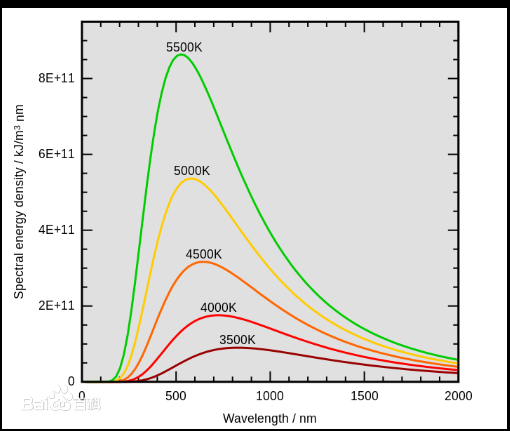
\includegraphics{img/black_body_radiators.png}}
\end{frame}}{\begin{frame}
  \
  
  \qquad\resizebox{0.8\columnwidth}{!}{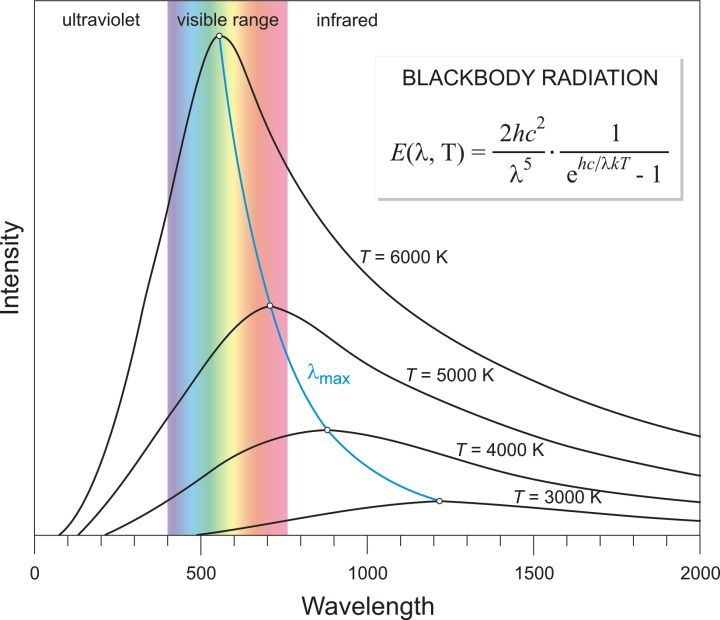
\includegraphics{img/black_body_radiators_color.jpg}}
\end{frame}}{\begin{frame}
  \frametitle{太阳与天空}
  
  {\hspace{4em}}\resizebox{0.7\columnwidth}{!}{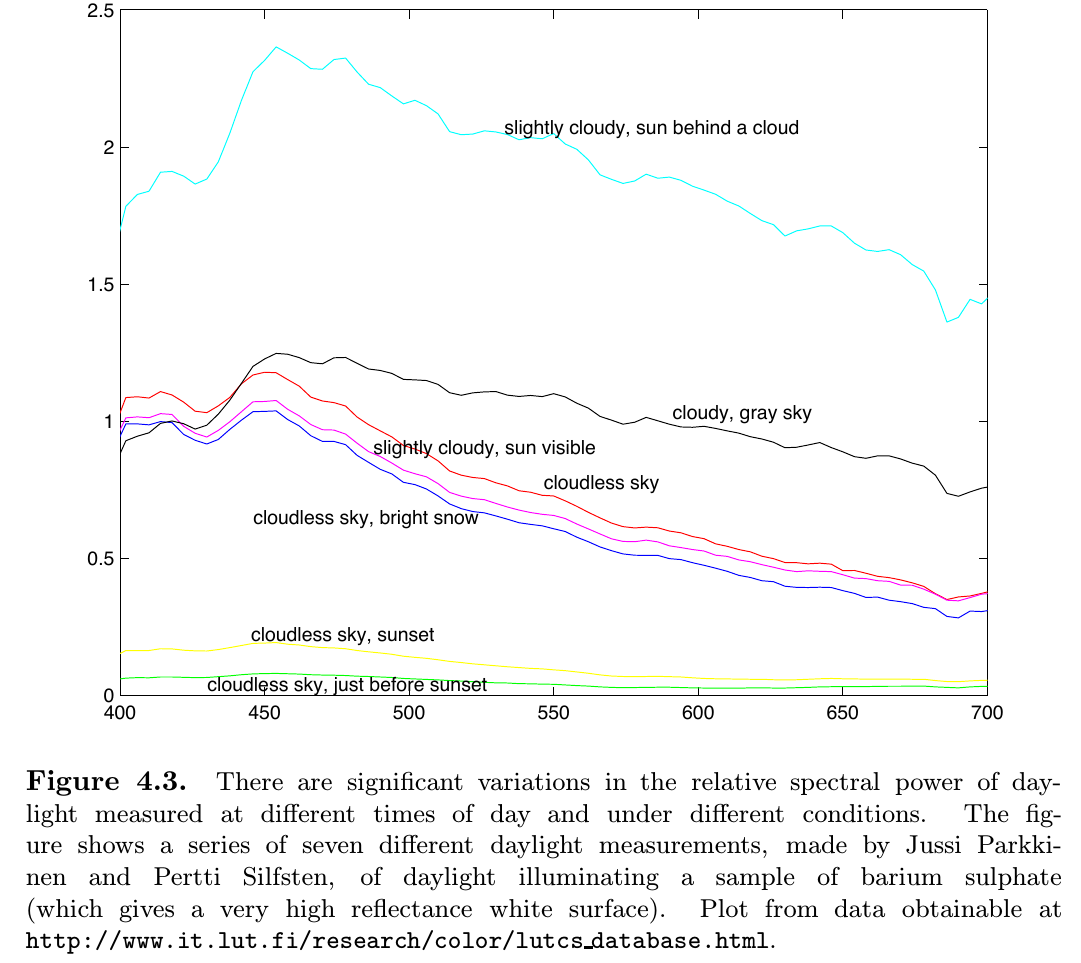
\includegraphics{img/day_light.png}}
\end{frame}}{\begin{frame}
  \frametitle{灯光}
  
  \qquad\resizebox{0.8\columnwidth}{!}{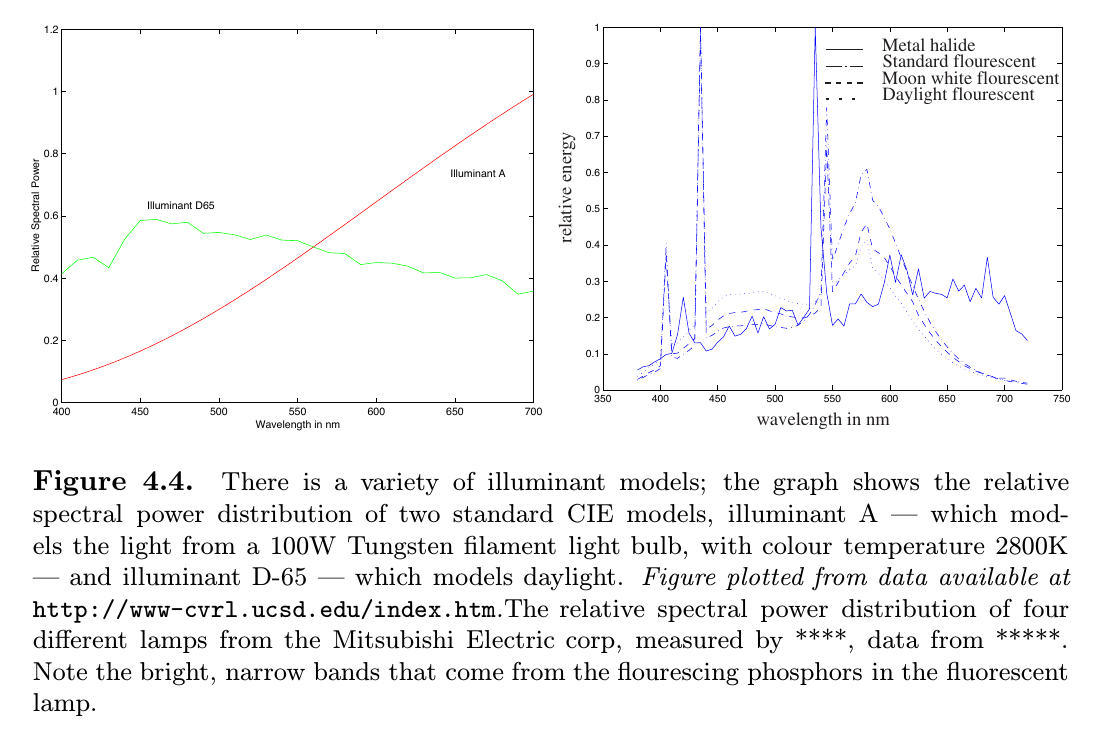
\includegraphics{img/illuminant_models.png}}
\end{frame}}{\begin{frame}
  \frametitle{表面的颜色}
  
  朗伯加镜面反射模型:
  \begin{eqnarray*}
    E (\lambda) & = & \rho_{\tmop{dh}} (\lambda) S (\lambda) \times
    \text{geometric terms} + \text{specular terms}
  \end{eqnarray*}
\end{frame}}{\begin{frame}
  \frametitle{光谱反射率------花与叶}
  
  \qquad\resizebox{0.9\columnwidth}{!}{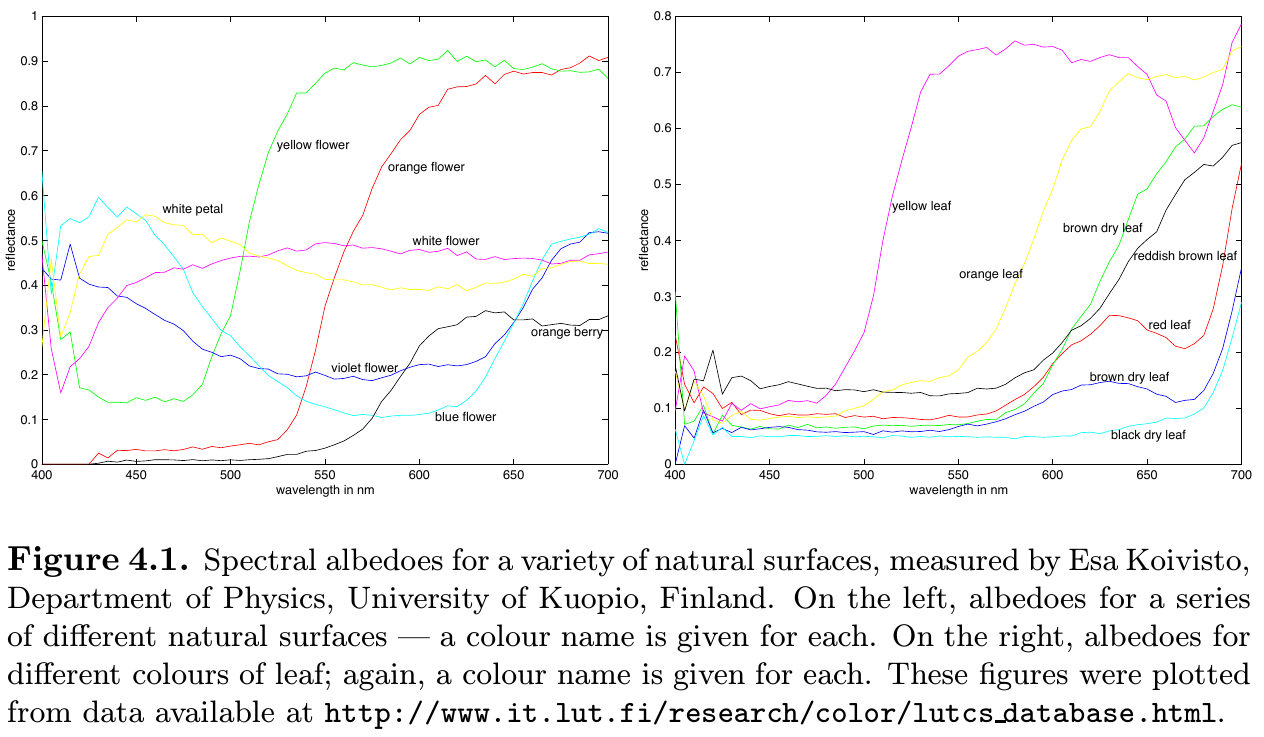
\includegraphics{img/spectral_albedoes_for_surfaces.png}}
\end{frame}}{\begin{frame}
  \frametitle{光谱反射率------红花与绿叶}
  
  \quad\resizebox{0.9\columnwidth}{!}{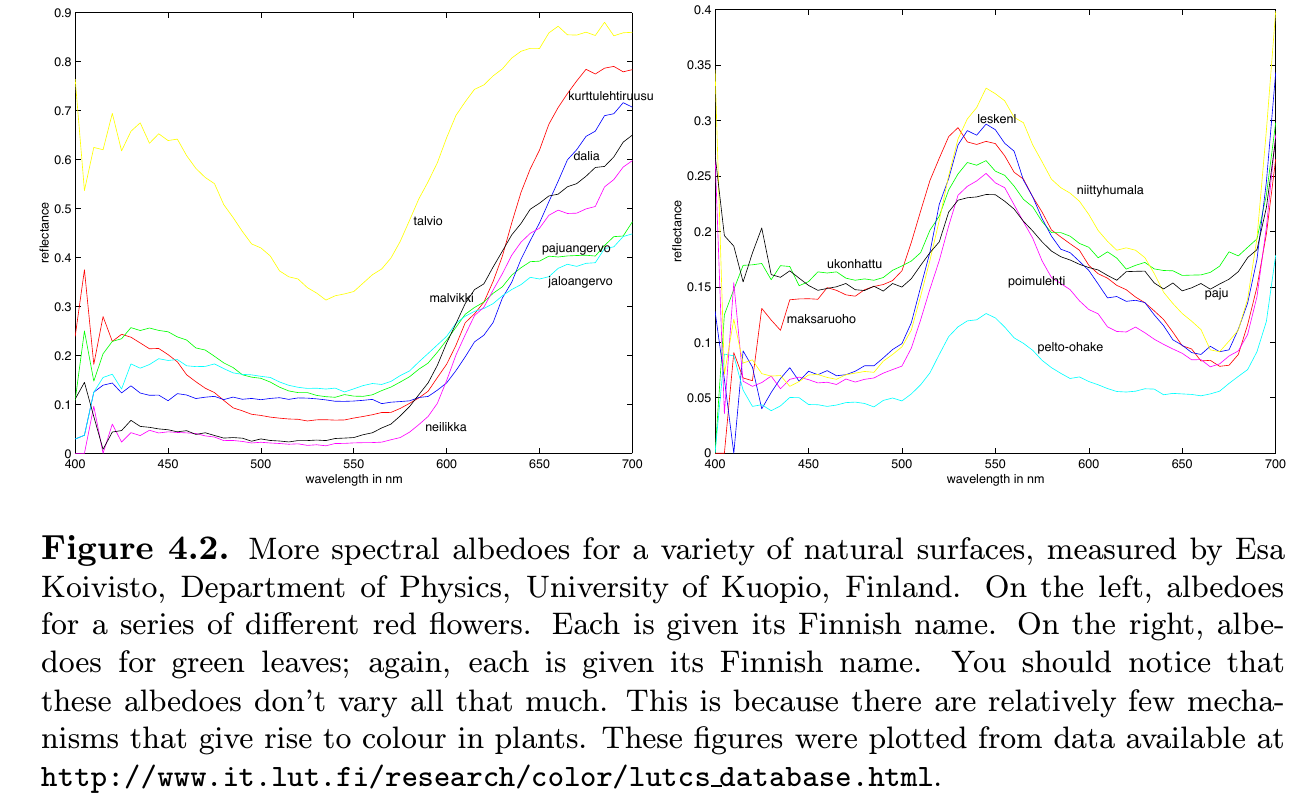
\includegraphics{img/more_spectral_albedoes_for_surfaces.png}}
  
  \ 
\end{frame}}{\begin{frame}
  \frametitle{颜色匹配}
  
  \quad\resizebox{0.9\columnwidth}{!}{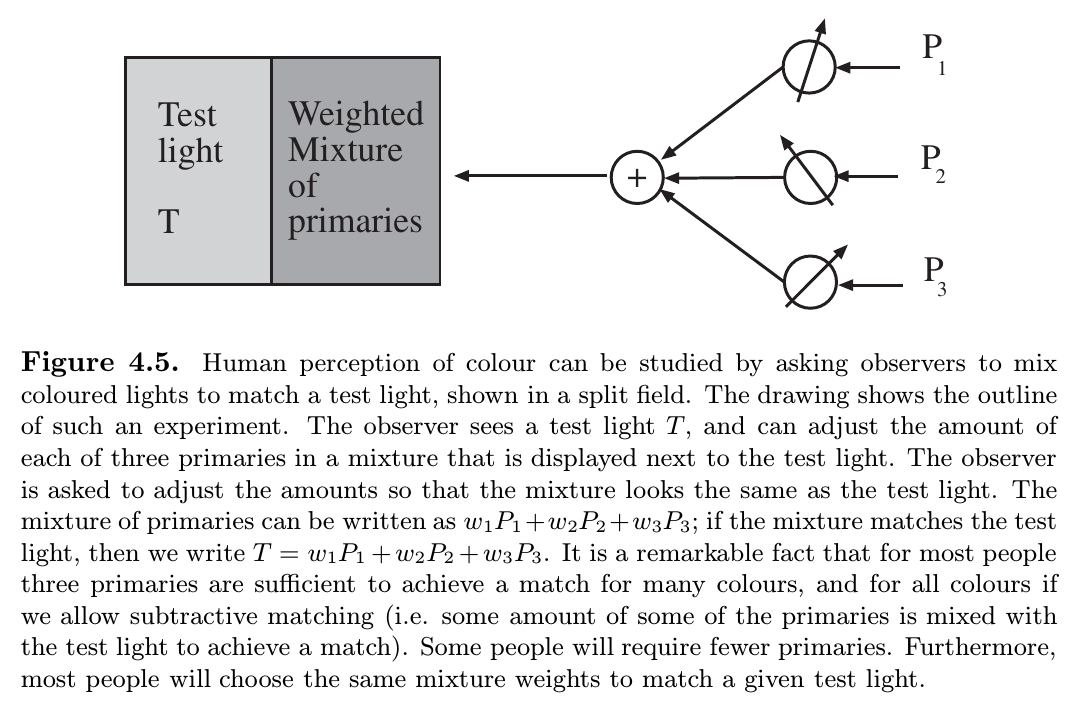
\includegraphics{img/color_match.png}}
\end{frame}}{\begin{frame}
  \frametitle{Grassman 定律}
  \begin{eqnarray*}
    T (\tmmathbf{w}) & = & \sum_i w_i P_i\\
    T (\tmmathbf{v}) & = & \sum_i v_i P_i\\
    T (k\tmmathbf{w}) + T (k\tmmathbf{v}) & = & k \nospace T
    (\tmmathbf{w}+\tmmathbf{v})
  \end{eqnarray*}
\end{frame}}{\begin{frame}
  \frametitle{颜色感受体}
  \begin{eqnarray*}
    p_k & = & \int_{\Lambda} \sigma_k (\lambda) E (\lambda) \mathd \lambda
  \end{eqnarray*}
  
\end{frame}}{\begin{frame}
  \frametitle{彩色视觉}
  
  \resizebox{364pt}{180pt}{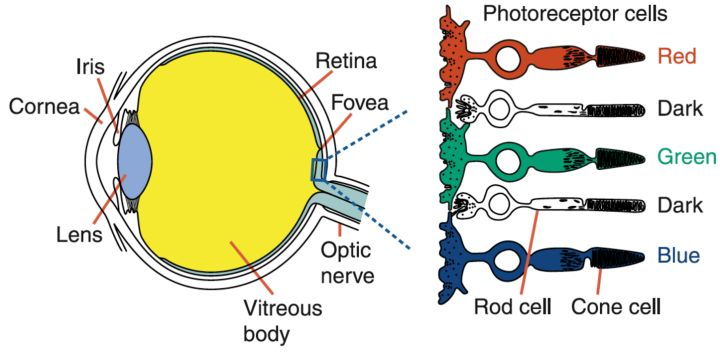
\includegraphics{img/human_eye_color_vision.jpg}}
\end{frame}}{\begin{frame}
  \frametitle{视锥细胞响应曲线}
  
  \quad\resizebox{0.9\columnwidth}{!}{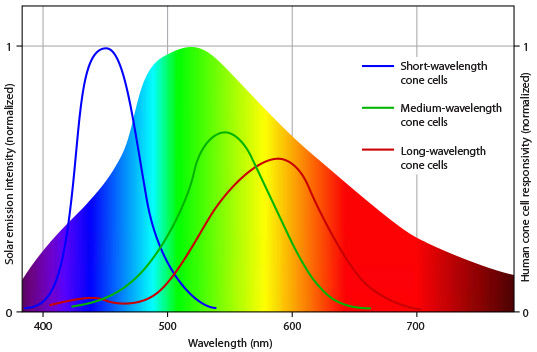
\includegraphics{img/cone_cell_response.jpg}}
\end{frame}}{\begin{frame}
  \frametitle{颜色匹配函数}
  
  
  \begin{eqnarray*}
    U (\lambda) & = & f_1 (\lambda) P_1 + f_2 (\lambda) P_2 + f_3 (\lambda)
    P_3\\
    S (\lambda) & = & \left( \int_{\Lambda} f_1 (\lambda) S (\lambda) \mathd
    \lambda \right) P_1 + \left( \int_{\Lambda} f_2 (\lambda) S (\lambda)
    \mathd \lambda \right) P_2 + \left( \int_{\Lambda} f_3 (\lambda) S
    (\lambda) \mathd \lambda \right) P_3
  \end{eqnarray*}
\end{frame}}{\begin{frame}
  \frametitle{线性颜色空间}
  
  \quad\resizebox{0.9\columnwidth}{!}{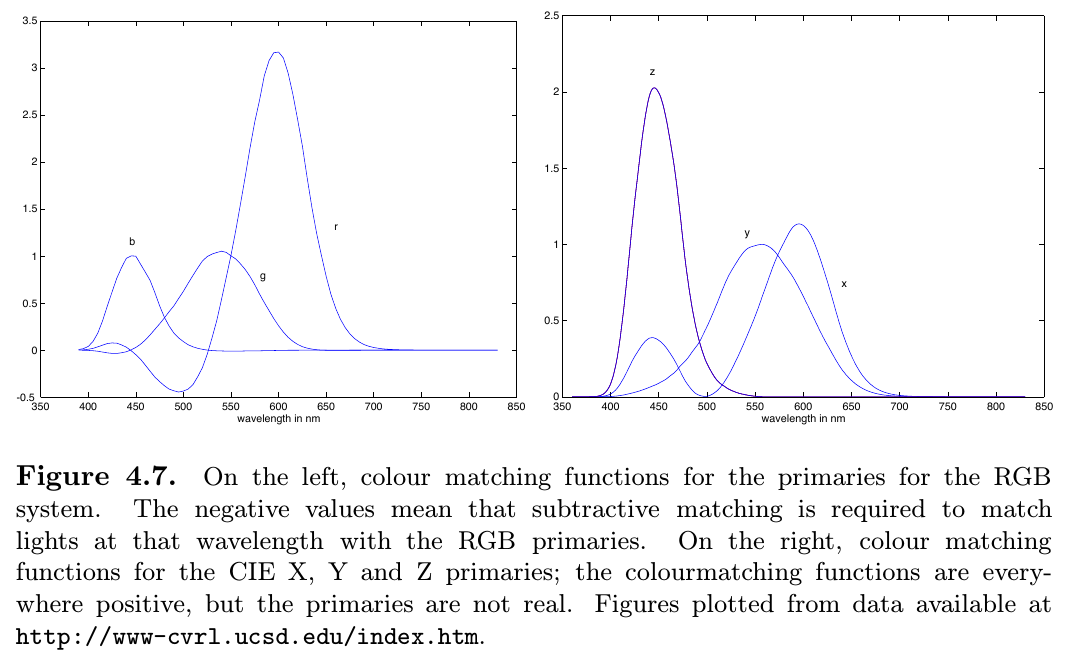
\includegraphics{img/RGB_CIE_XYZ.png}}
\end{frame}}{\begin{frame}
  \frametitle{CIE XYZ颜色空间}
  
  {\hspace{3em}}\resizebox{0.8\columnwidth}{!}{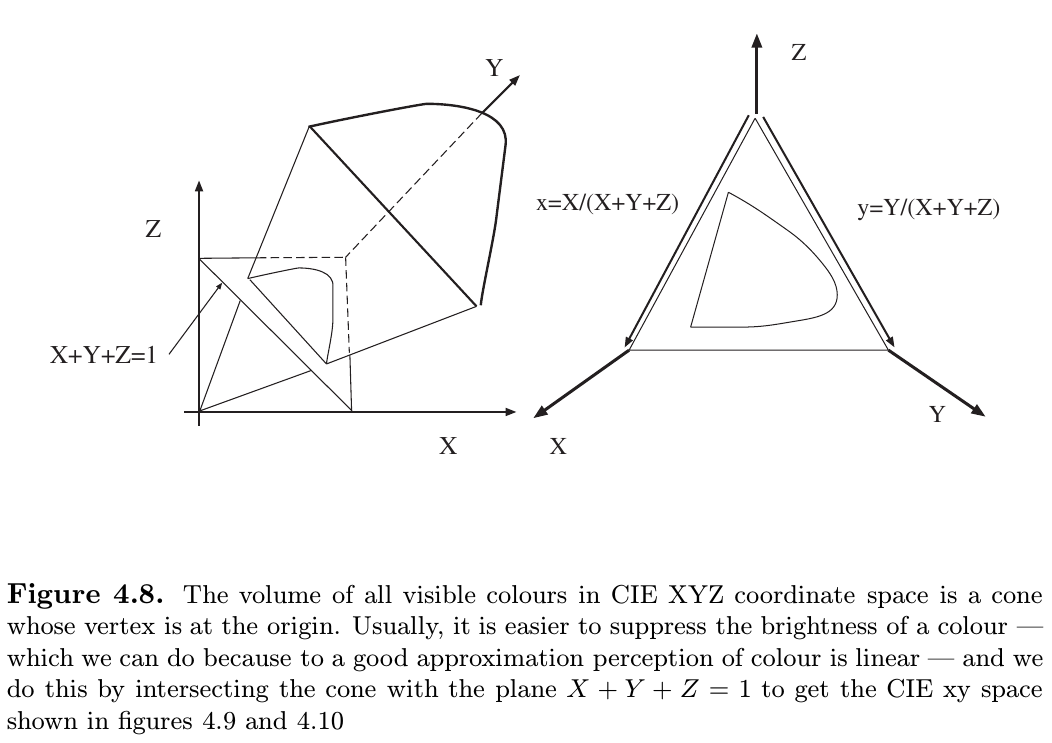
\includegraphics{img/CIE_XYZ.png}}
\end{frame}}{\begin{frame}
  \frametitle{CIE xy}
  
  {\hspace{5em}}\resizebox{0.6\columnwidth}{0.6\columnwidth}{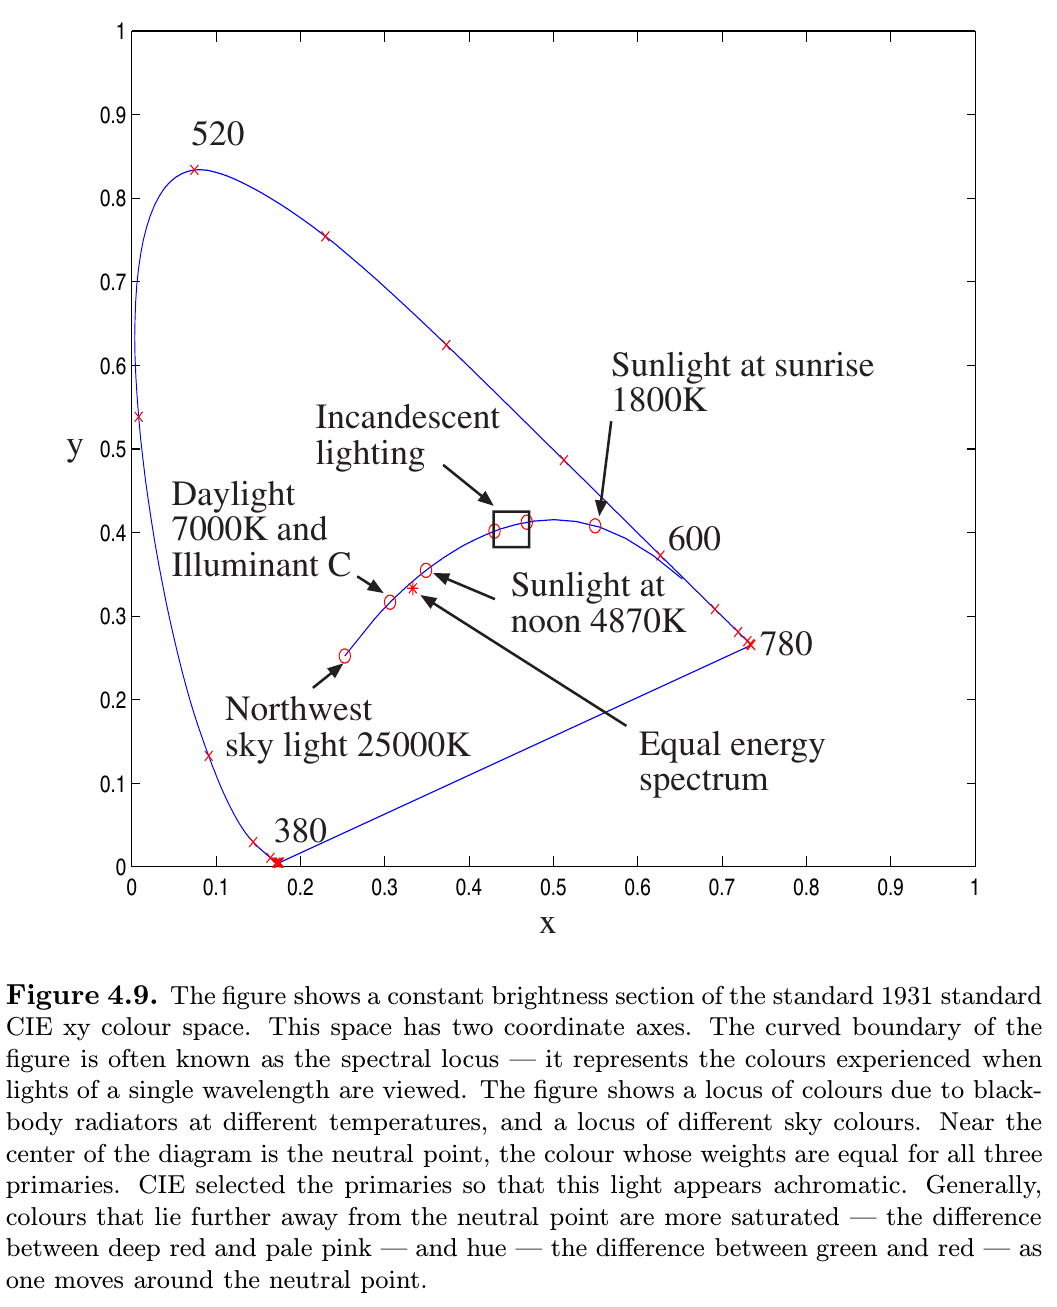
\includegraphics{img/CIE_xy.png}}
\end{frame}}{\begin{frame}
  \frametitle{Saturation \& Hue}
  
  {\hspace{6em}}\resizebox{0.5\columnwidth}{!}{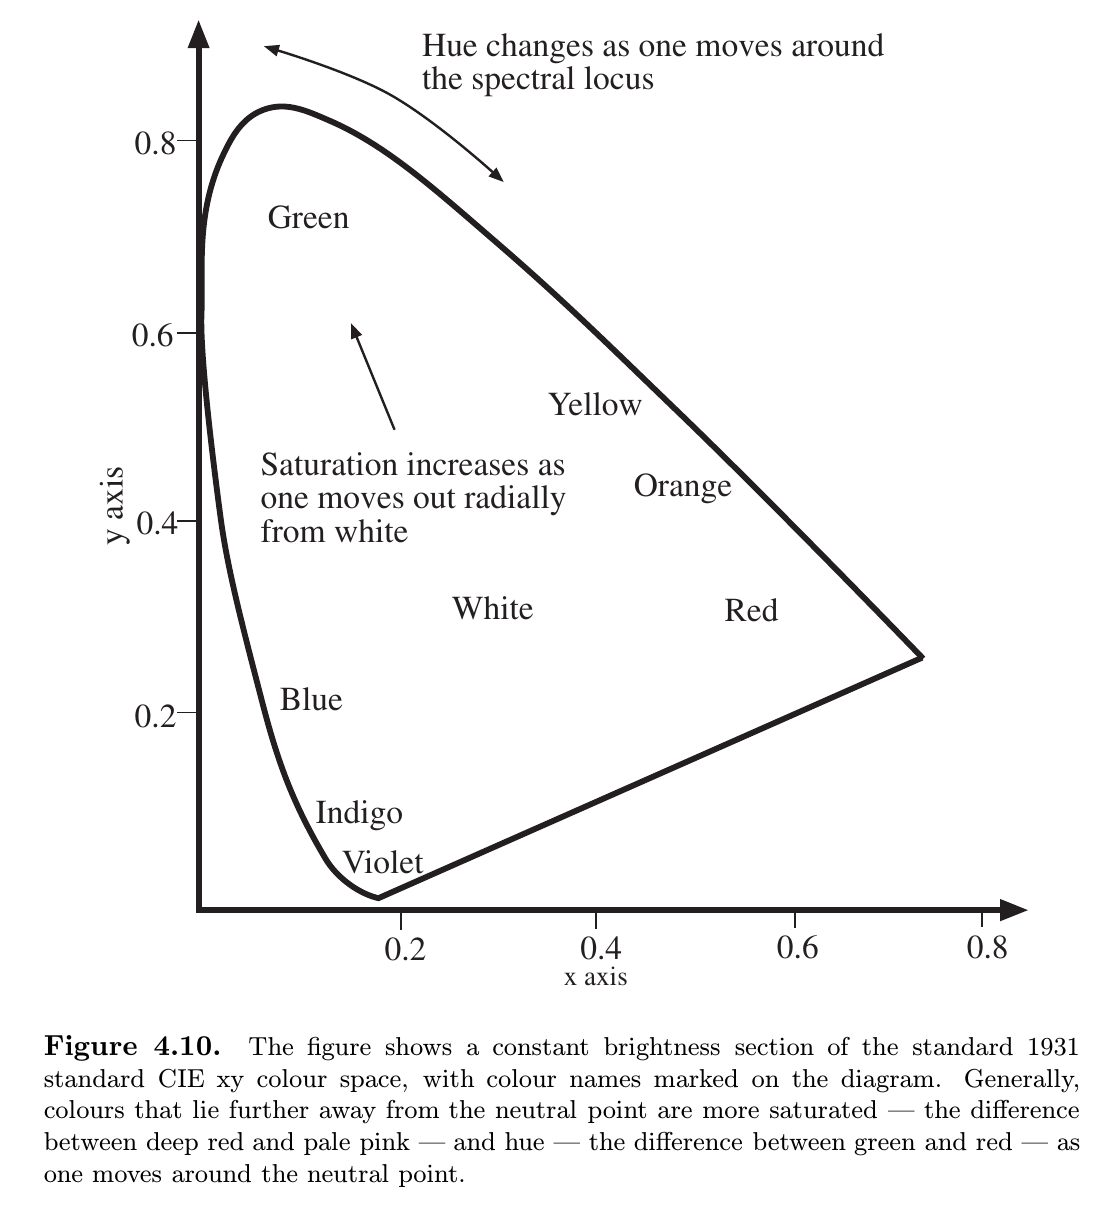
\includegraphics{img/saturation_hue.png}}
\end{frame}}{\begin{frame}
  \frametitle{颜色混合}
  
  {\hspace{4em}}\resizebox{0.7\columnwidth}{!}{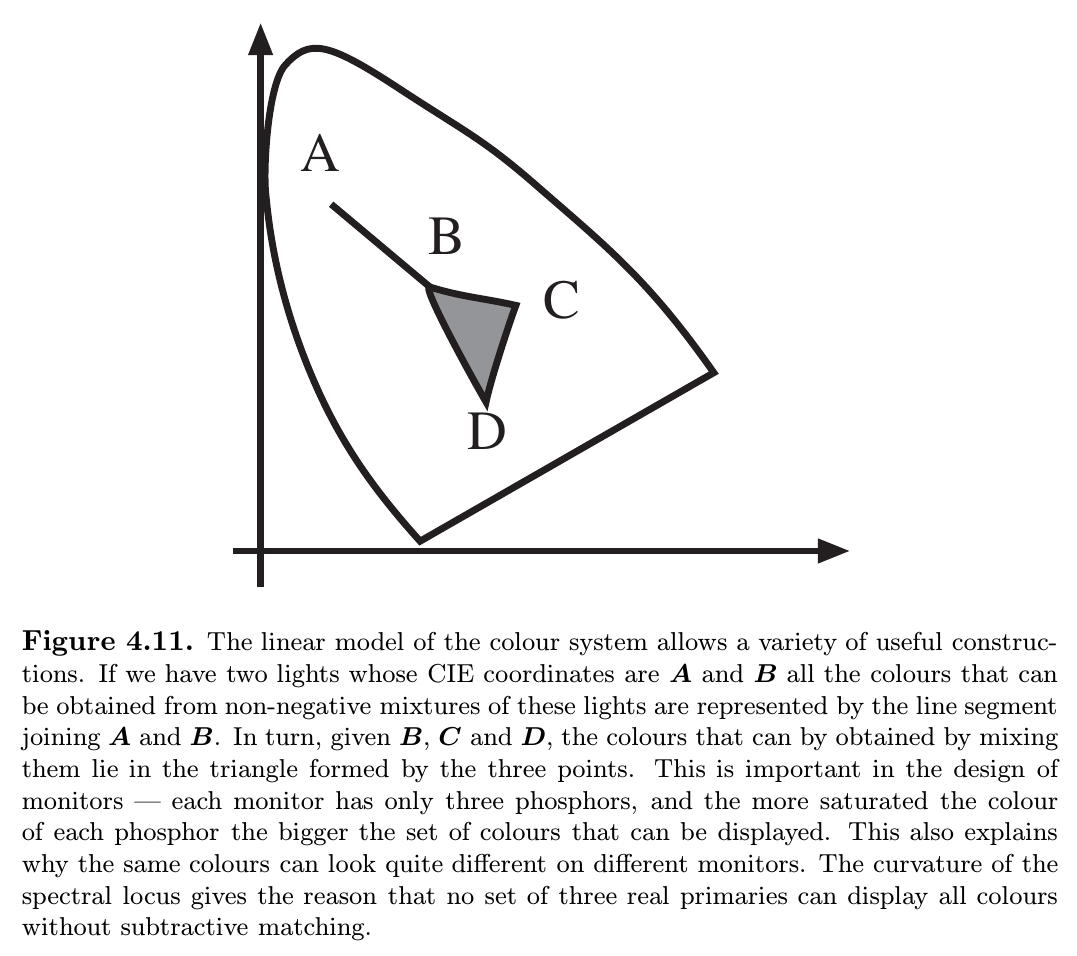
\includegraphics{img/mixing_color.png}}
\end{frame}}{\begin{frame}
  \frametitle{RGB颜色空间}
  
  \resizebox{1\columnwidth}{!}{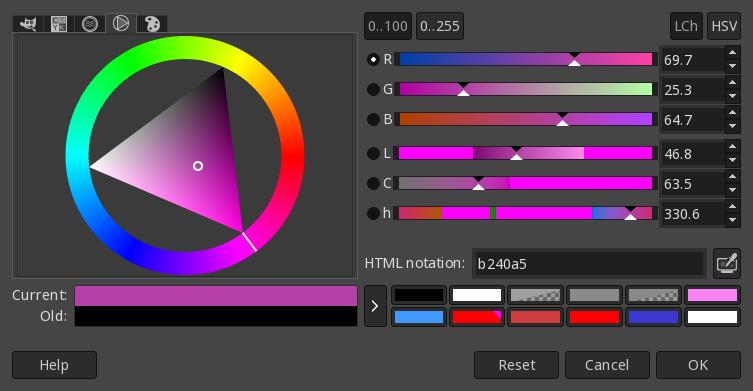
\includegraphics{img/rgb_lch.png}}
\end{frame}}{\begin{frame}
  \frametitle{CMYK颜色空间}
  \begin{itemizedot}
    \item cyan (a blue-green colour) = W -- R (white -- red);
    
    \item magenta (a purplish colour) = W -- G (white -- green)
    
    \item  and yellow = W -- B (white -- blue)
  \end{itemizedot}
\end{frame}}{\begin{frame}
  \frametitle{Hue, Saturation and Value}
  
  \qquad\resizebox{0.8\columnwidth}{!}{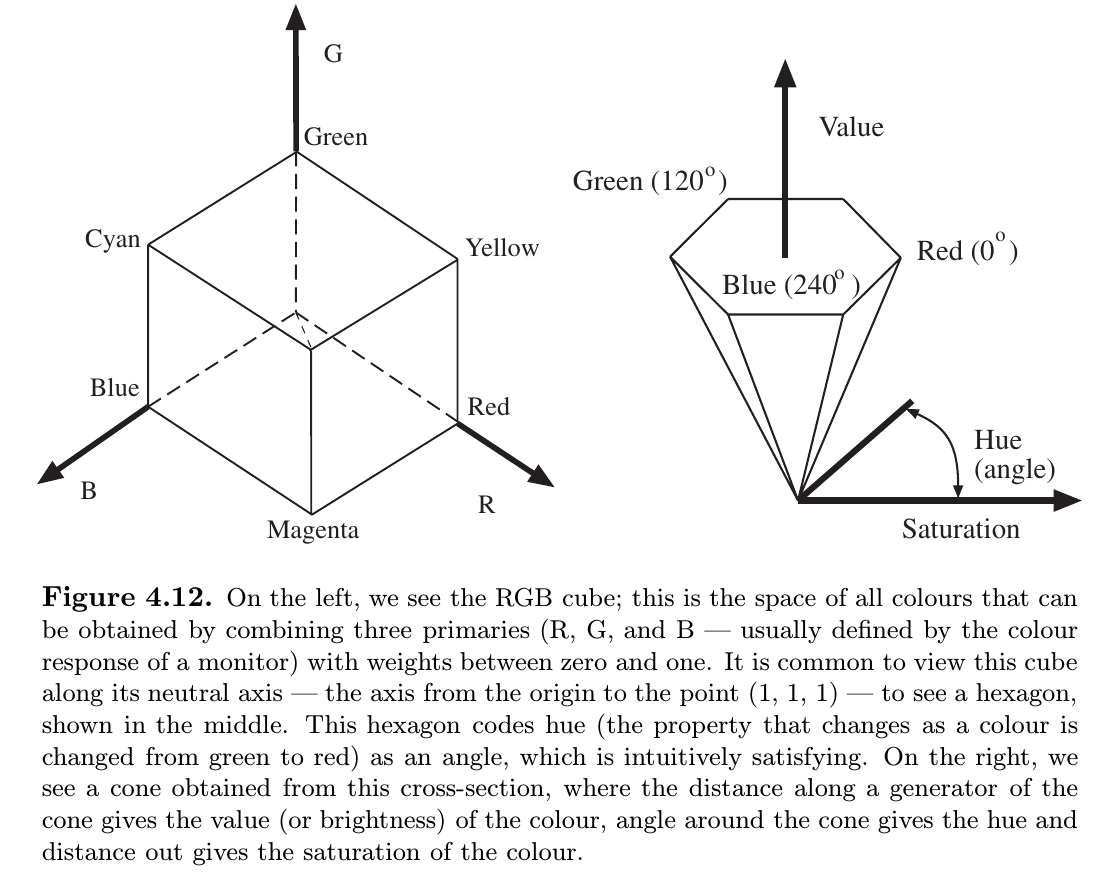
\includegraphics{img/rgb_hsv.png}}
\end{frame}}{\begin{frame}
  \frametitle{均匀颜色空间}
  
  {\hspace{4em}}\resizebox{0.7\columnwidth}{!}{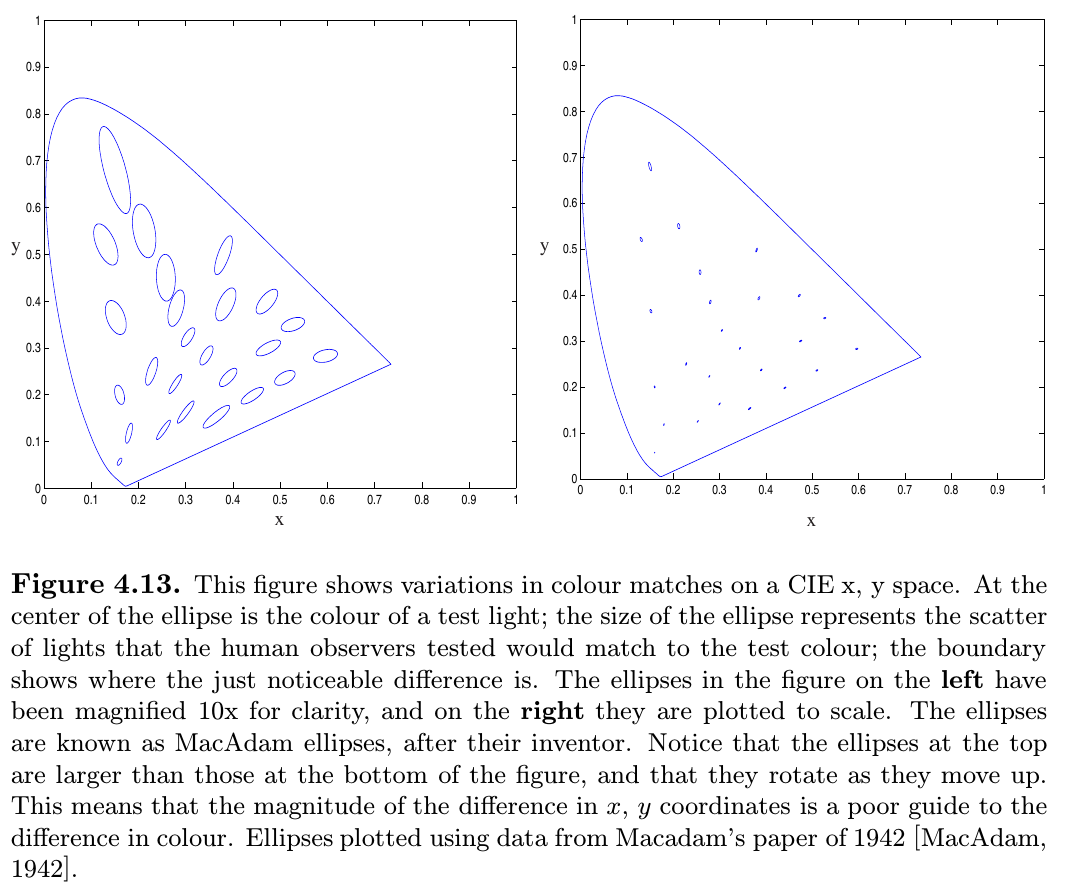
\includegraphics{img/just_noticeable_difference.png}}
\end{frame}}{\begin{frame}
  \frametitle{CIE u'v'颜色空间}
  
  {\hspace{3em}}\resizebox{0.8\columnwidth}{!}{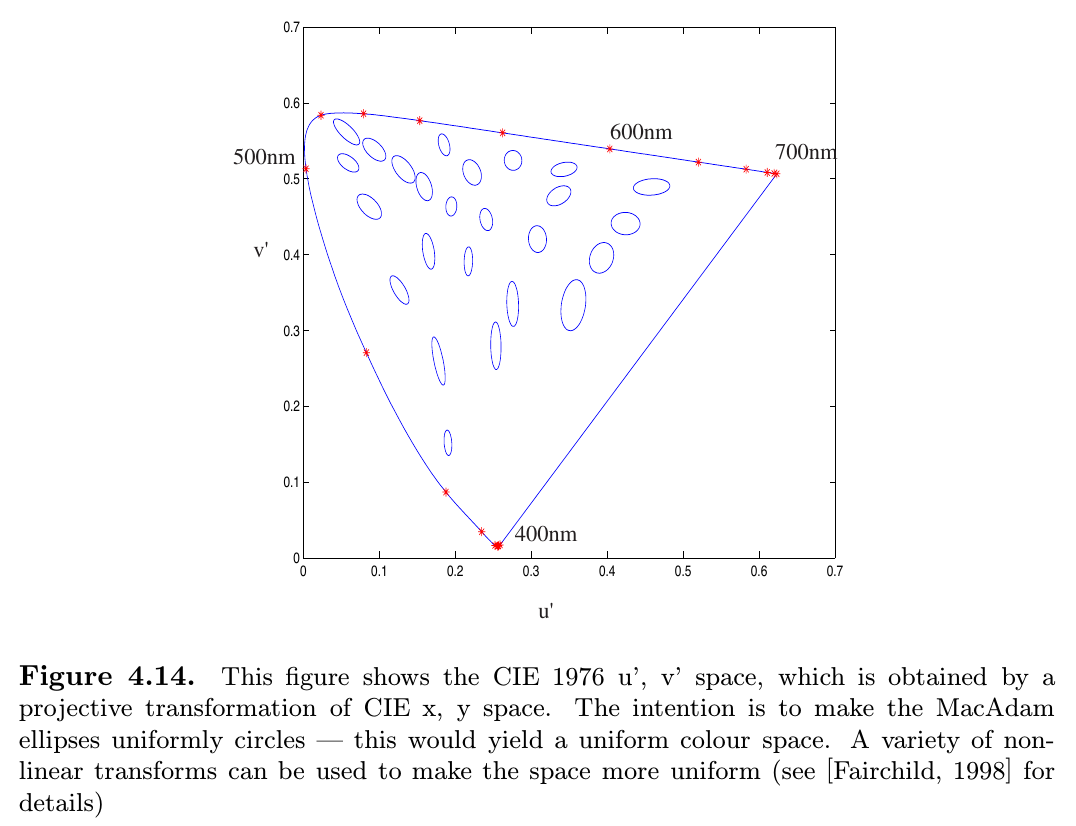
\includegraphics{img/CIE_uv.png}}
\end{frame}}{\begin{frame}
  \frametitle{CIE LAB颜色空间}
  \begin{eqnarray*}
    L^{\ast} & = & 116 \left( \frac{Y}{Y_n} \right)^{\frac{1}{3}} - 16\\
    a^{\ast} & = & 500 \left( \left( \dfrac{X}{X_n} \right)^{\frac{1}{3}} -
    \left( \dfrac{Y}{Y_n} \right)^{\frac{1}{3}} \right)\\
    b^{\ast} & = & 200 \left( \left( \frac{Y}{Y_n} \right)^{\frac{1}{3}} -
    \left( \frac{Z}{Z_n} \right)^{\frac{1}{3}} \right)
  \end{eqnarray*}
\end{frame}}{\begin{frame}
  \frametitle{图像颜色模型}
  
  \quad\resizebox{0.9\columnwidth}{!}{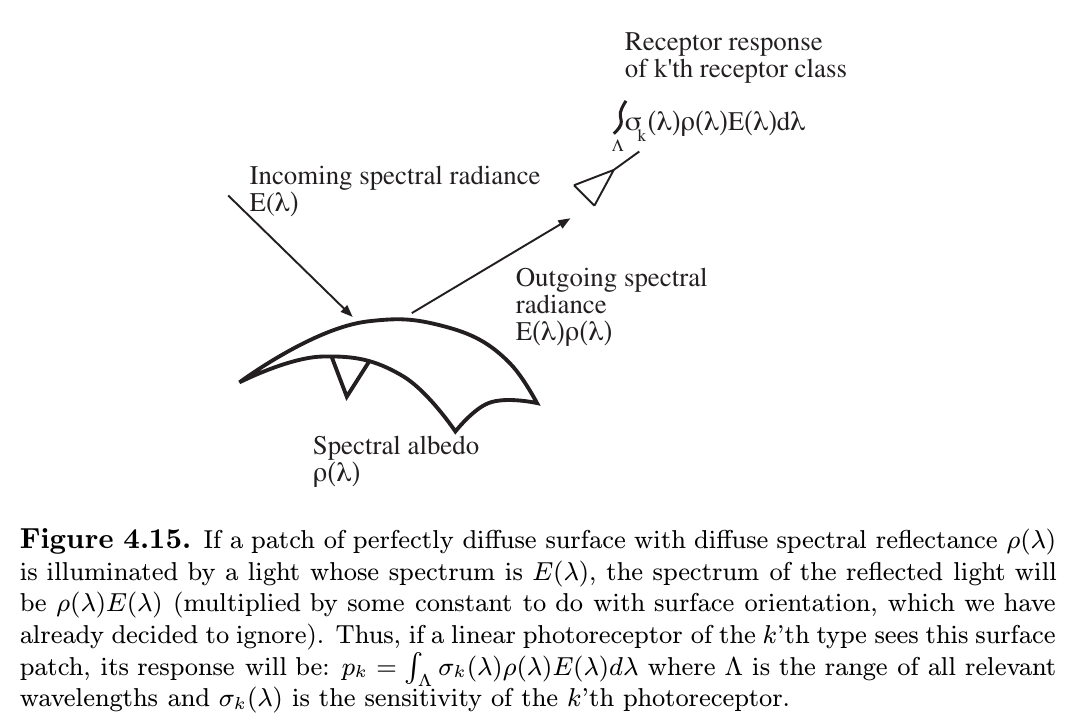
\includegraphics{img/patch_color.png}}
\end{frame}}{\begin{frame}
  \frametitle{}
  
  
  \begin{eqnarray*}
    \tmmathbf{C} (\tmmathbf{x}) & = & (\tmop{diffuse} \tmop{term}) +
    (\tmop{specular} \tmop{term})\\
    & = & (\tmop{direct} \tmop{term}) + (\tmop{interreflected} \tmop{term}) +
    (\tmop{specular} \tmop{term})\\
    & = & g_d (\tmmathbf{x}) \tmmathbf{d} (\tmmathbf{x}) +\tmmathbf{i}
    (\tmmathbf{x}) + g_s (\tmmathbf{x}) \tmmathbf{s} (\tmmathbf{x})
  \end{eqnarray*}
  $\tmmathbf{d} (\tmmathbf{x})$模型:
  \begin{eqnarray*}
    p_k & = & \int_{\Lambda} \sigma_k (\lambda) \rho (\lambda) S (\lambda)
    \mathd \lambda
  \end{eqnarray*}
\end{frame}}{\begin{frame}
  \frametitle{漫反射与镜面反射}
  
  {\hspace{5em}}\resizebox{0.6\columnwidth}{!}{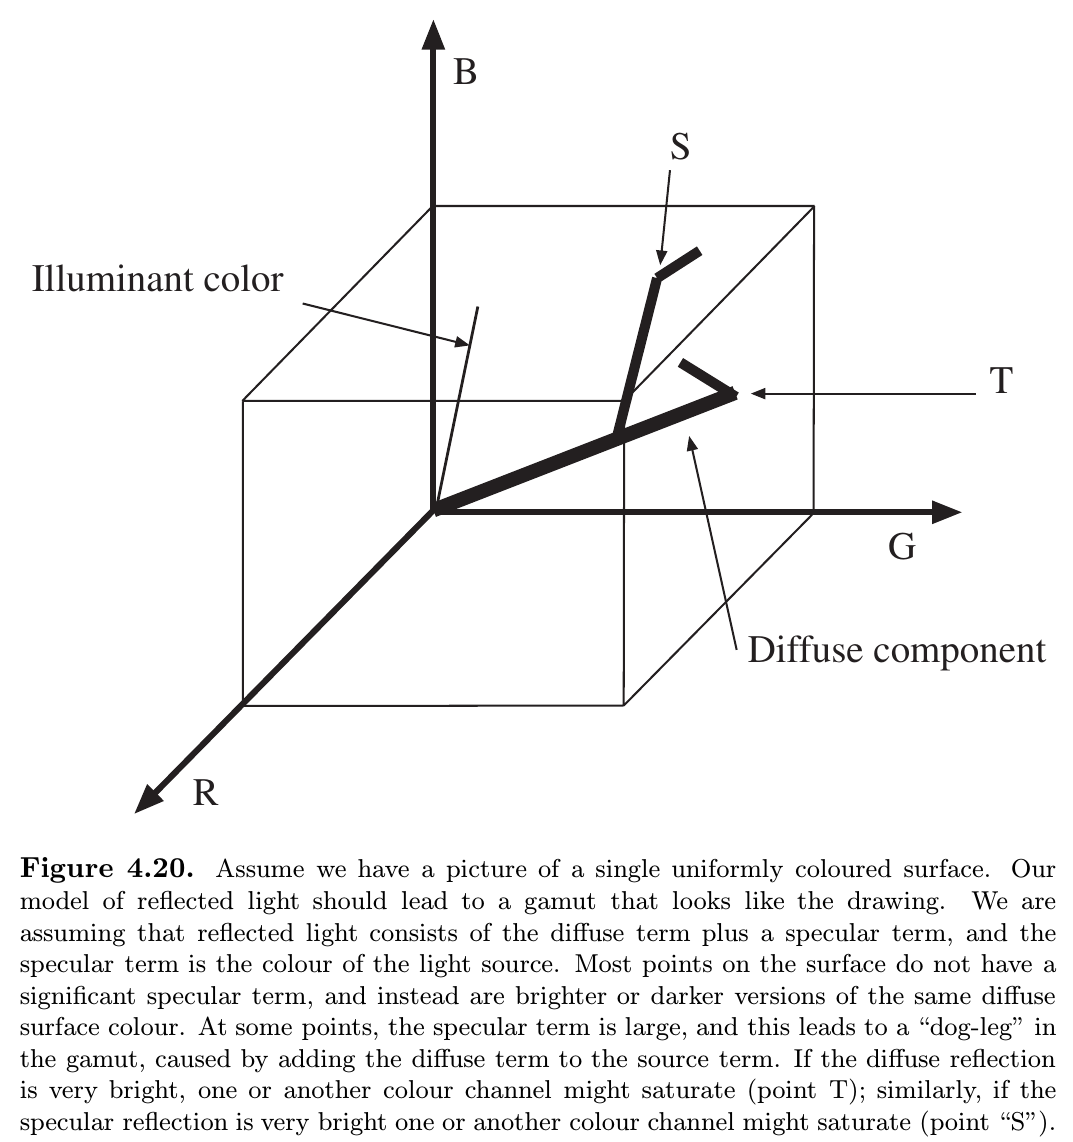
\includegraphics{img/diffuse_specular.png}}
\end{frame}}{\begin{frame}
  \frametitle{找到镜面反射}
  
  {\hspace{7em}}\resizebox{0.5\columnwidth}{!}{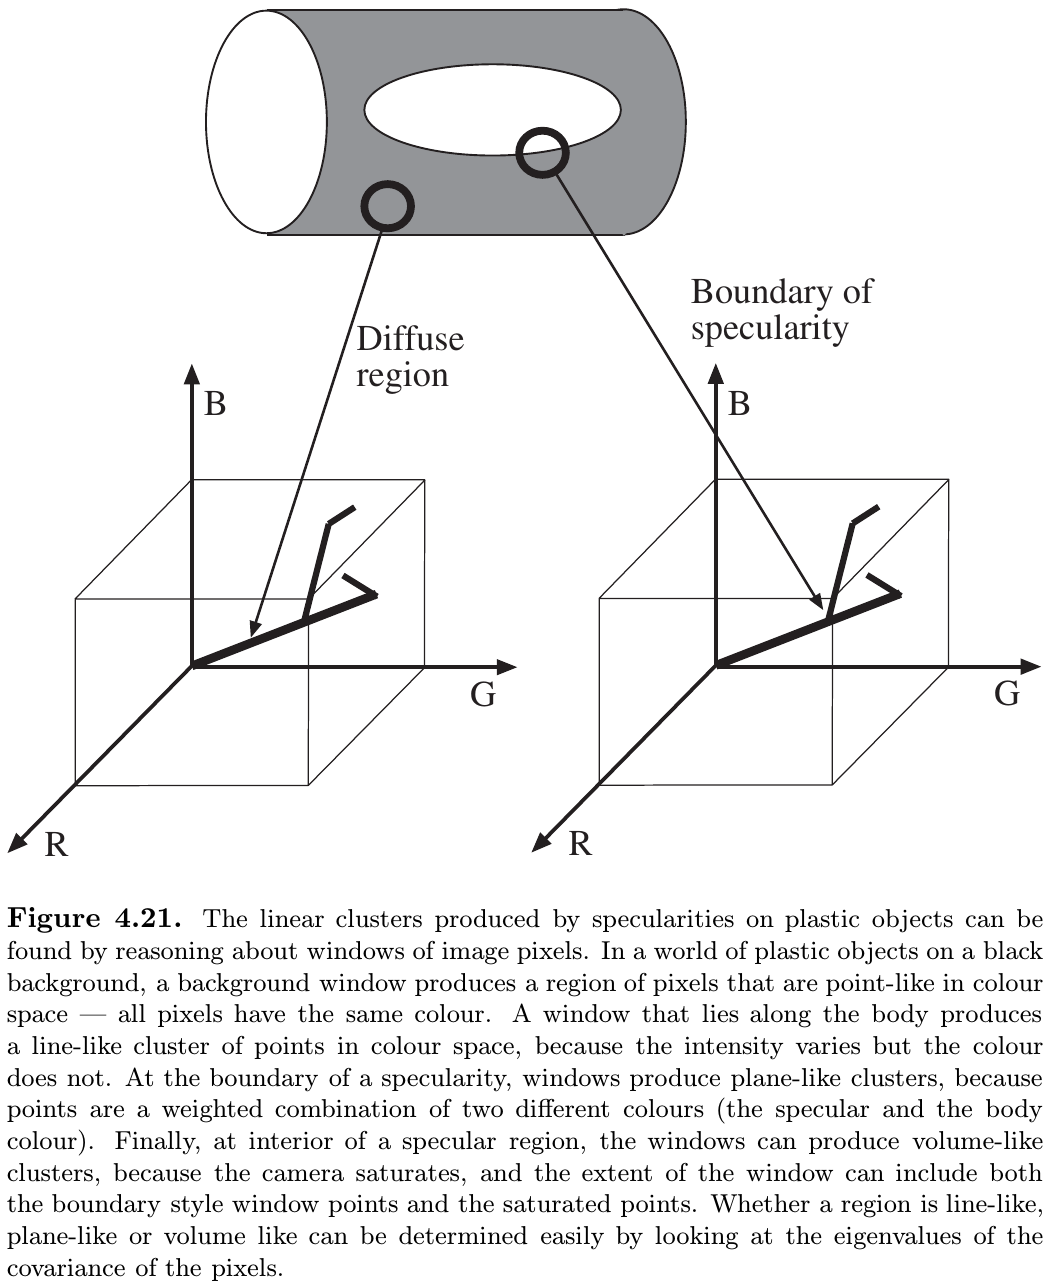
\includegraphics{img/find_specular.png}}
\end{frame}}{\begin{frame}
  \frametitle{阴影消除}
  \begin{eqnarray*}
    E (\lambda ; T) & = & K \lambda^{- 5} e^{\frac{- h \nospace c}{k \lambda
    T}}\\
    \sigma_k (\lambda) & = & \delta (\lambda - \lambda_k)\\
    r_j & = & \int \sigma_j (\lambda) \rho (\lambda) K \lambda^{- 5}
    e^{\frac{- h \nospace c}{k \lambda T}} \mathd \lambda\\
    & = & K \rho (\lambda) \lambda_j^{- 5} e^{\frac{- h \nospace c}{k
    \lambda_j T}}
  \end{eqnarray*}
  
  
  \ 
\end{frame}}{\begin{frame}
  \frametitle{颜色空间}
  \begin{eqnarray*}
    &  & 
  \end{eqnarray*}
  
  \begin{eqnarray*}
    c_1 & = & \log \left( \frac{r_1}{r_3} \right)\\
    c_2 & = & \log \left( \frac{r_2}{r_3} \right)\\
    \left(\begin{array}{c}
      c_1\\
      c_2
    \end{array}\right) & = & \left(\begin{array}{c}
      a_1\\
      a_2
    \end{array}\right) + \frac{1}{T} \left(\begin{array}{c}
      b_1\\
      b_2
    \end{array}\right)
  \end{eqnarray*}
\end{frame}}{\begin{frame}
  \frametitle{颜色方向}
  
  \quad\resizebox{0.9\columnwidth}{!}{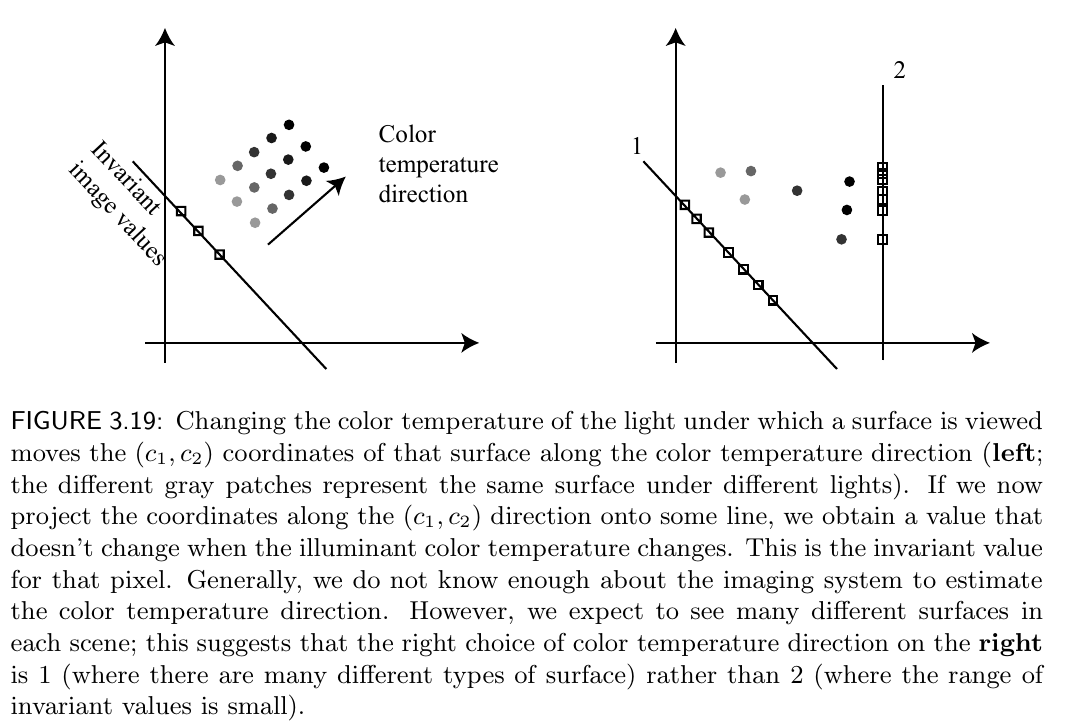
\includegraphics{img/color_direction.png}}
\end{frame}}{\frametitle{颜色恒常性}

\qquad\resizebox{0.8\columnwidth}{!}{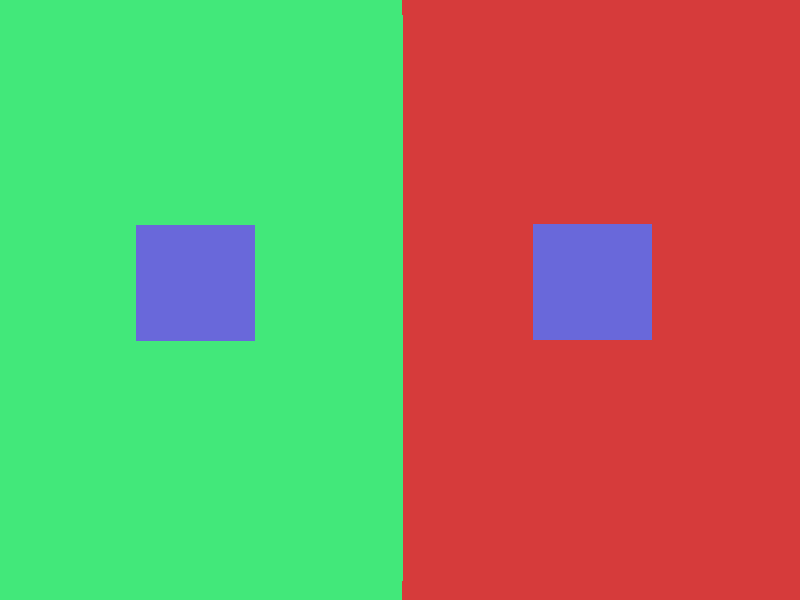
\includegraphics{img/color_constancy.png}}}{\begin{frame}
  \frametitle{有限维线性模型}
  \begin{eqnarray*}
    \rho (\lambda) & = & \sum_{j = 1}^n r_j \varphi_j (\lambda)\\
    E (\lambda) & = & \sum_{i = 1}^m e_i \psi_i (\lambda)\\
    p_k & = & \int \sigma_k (\lambda) \left( \sum_{j = 1}^n r_j \varphi_j
    (\lambda) \right) \left( \sum_{i = 1}^m e_i \psi_i (\lambda) \right)
    \mathd \lambda\\
    & = & \sum_{j = 1}^n \sum_{i = 1}^m e_i r_j \int \sigma_k (\lambda)
    \varphi_j (\lambda) \psi_i (\lambda) \mathd \lambda\\
    & = & \sum_{j = 1}^n \sum_{i = 1}^m e_i r_j g_{i \nospace j \nospace k}
  \end{eqnarray*}
\end{frame}}{\begin{frame}
  \frametitle{推断表面颜色(镜面反射率相同)}
  
  己知$\sigma_k, \psi_i$求$e_i$:
  \begin{eqnarray*}
    p_k & = & \int \sigma_k (\lambda) \sum_{i = 1}^m e_i \psi_i (\lambda)
    \mathd \lambda\\
    & = & \sum_{i = 1}^m \sum_{j = 1}^n \int \sigma_k (\lambda) e_i \psi_i
    (\lambda) \mathd \lambda
  \end{eqnarray*}
  $r_j$:
  \begin{eqnarray*}
    p_k & = & \sum_{j = 1}^n \sum_{i = 1}^m e_i r_j g_{i \nospace j \nospace
    k}
  \end{eqnarray*}
\end{frame}}{\begin{frame}
  \frametitle{推断表面颜色(平均反射率是常数)}
  
  已知$\overline{p}_k, \overline{r}_j$, 求$e_i$
  \begin{eqnarray*}
    \overline{\rho} & = & \sum_{j = 1}^n \overline{r}_j \varphi_j (\lambda)\\
    \overline{p}_k & = & \sum_{j = 1}^n \sum_{i = 1}^m e_i g_{i \nospace j
    \nospace k} \overline{r}_j
  \end{eqnarray*}
  $r_j$:
  \begin{eqnarray*}
    p_k & = & \sum_{j = 1}^n \sum_{i = 1}^m e_i r_j g_{i \nospace j \nospace
    k}
  \end{eqnarray*}
\end{frame}}}

\end{document}
